%
%  Simulations
% =============
%

\chapter{Simulations}
\label{Ch:Sim}

The work presented in this thesis has been performed using simulations with two particle-in-cell (PIC) codes:
OSIRIS \cite{fonseca:2002} and QuickPIC \cite{an:2013, huang:2006}.
OSIRIS is a proprietary full PIC code available in 1, 2 and 3 dimensions, with a choice between Cartesian and cylindrical coordinates.
QuickPIC is a quasi-static 3D PIC code. In this work the open source version of QuickPIC has been used \cite{add:quickpic:web}.
For a more detailed description on PIC codes, see Appendix \ref{Apx:PIC}.

Although PIC codes use macro particles -- that is, simulated particles represent more than one physical beam or plasma particle -- these codes require a lot of CPU power.
This is especially true when running in 3D.
The preliminary studies presented in Publications \ref{Pub:IPAC15} and \ref{Pub:NAPAC16} were done using OSIRIS with 2D cylindrical coordinates.
The main study, Publication \ref{Pub:BL17}, was done using QuickPIC in 3D.
In order to perform the detailed parameter scans needed for these studies, the drive beam and accelerating structure had to be scaled down into a more manageable size than the full SPS proton beam.
This chapter will outline the simulation environment chosen for these studies, and the reasons behind these.

% ================================================================================================================================ %
\section{Simulating the Drive Bunch}
\label{Sim:PBeam}

An initial set of simulations were run to study the evolution of the self-modulation instability in the SPS proton bunch.
These simulations assumed the plasma was ionised at the centre of the bunch, so only the back half of it was actually simulated.
The beam profile function thus took the form:
\begin{equation}
    f(\xi,r) = \frac{A}{2} \left[1 + \cos\left(\xi\frac{\pi}{L}\right)\right] \exp\left(-\frac{r^{2}}{2\sigma_{r}^{2}}\right), \label{EQ:SPS-Profile}
\end{equation}
where $L = 2.5\sigma_{z,pb} = 30\unit{cm}$ is the length of half an SPS proton bunch, $R$ is the radius of the simulation box, and $A_{q}$ is a charge scaling factor to match the SPS bunch charge.
The total charge of the simulated proton bunch in cylindrical coordinates is thus given by:
\begin{equation}
    Q_{pb} = 2\pi \iint f(\xi,r) \;r \deriv r \deriv \xi, \label{EQ:SPS-Charge}
\end{equation}
where $A$ is tuned such that $Q_{pb}$ matches the charge outlined in Table \ref{T:AWAKE-Run1}.
A half period cosine function for the longitudinal density profile is more convenient for simulations than a Gaussian shape, as the cosine goes to zero at a finite length \cite{lotov:2010}.

% ================================================================================================================================ %

\subsection{With a Pre-Modulated Beam}
\label{Sim:PBPreMod}

In order to make the simulations more manageable in size for the beam loading studies, we decided to move to a sample proton beam of $26$ micro bunches.
These simulations were all done using OSIRIS 3.0.
With this version it is necessary for the beams to drift in vacuum for a short distance for the electro-magnetic fields to develop properly, as they are initialised at zero (see further discussion in Section \ref{PIC:Full}).
Since the evolution of the self-modulation instability was not of primary interest at this stage, we chose to modify the beam profile to emulate a section of the modulated bunch.
We refer to this as \textit{pre-modulation}.
This was done by shortening the period of the density envelope cosine function in Eq. \ref{EQ:SPS-Profile} to match that of the plasma wavelength.
\begin{equation}
    f(\xi,r) = A\sqrt{2} \left[\frac{1}{2\sqrt{2}}
             + \cos\left(k_{pe}\xi - \mu\right)\right] \exp\left(-\frac{r^{2}}{2\sigma_{r}^{2}}\right), \label{EQ:PB-PreMod}
\end{equation}
where $\mu$ is the position of the first micro bunch, and $k_{pe}$ is the plasma wave number \cite{berglyd_olsen:2015}.
The offset of the cosine function is chosen such that the width of the micro bunch matches the width of a bunch in the simulations done with a full bunch.
Since OSIRIS ignores profile densities with negative values, the profile is automatically clipped at $0$.

Again, cosines are preferred over a series of Gaussian bunch profiles.
As before, they have clearly defined end points, but also due to limitations in the input files of OSIRIS.
Mathematical functions are limited by the simulation software to $256$ characters.

% Comment about the separation between bunch 1 and 2?

The charge of the proton micro-bunches were matched to that of a micro-bunch generated by the self-modulation instability in the initial simulations.
This charge, of course, decreases towards the back end of the modulated beam, so they were fixed to a charge for the region were the injection of an electron bunch is reasonable.
For the pre-modulated simulations, this number was set to $100\unit{pC}$ such that the total charge of the sample proton beam was $2.6\unit{nC}$.
This corresponds to a peak current of $135\unit{A}$.
The electron witness bunch was injected between bunch $20$ and $21$.


% ================================================================================================================================ %

\subsection{With a Single Drive Bunch}
\label{Sim:PBSingle}

Text

% ================================================================================================================================ %
\section{Simulating the Witness Bunch}
\label{Sim:EBeam}

There were a few points to consider when simulating the electron witness beam.
These challenges differ between the two simulation codes used in these studies.

% ================================================================================================================================ %
\subsection{Witness Bunch Size and Resolution}
\label{Sim:EBeam:SizeRes}

For the early simulations, a transverse size of $\sigma_{x,y}=105\unit{\mu m}$ was used, see Table~\ref{T:AWAKE-Run2}.
For later simulations, when the beam transverse size was matched to its emittance and the plasma density (see Section \ref{Int:BPI:Match}), much narrower beams were used -- on the order of a few micrometres.
The proton drive beam size is tied to the plasma skin depth (see Section~\ref{Int:DBeam:SMI}), which is $200\unit{\mu m}$.
This, naturally, poses a resolution challenge when very narrow electron beams need to be resolved while the simulation box needs to be able to contain the proton drive bunch.

For the simulations with a pre-modulated proton beam, used for Publication~\ref{Pub:IPAC15}, the simulation box had a radius of $2.12\unit{mm}$ with $425$ grid cells, resulting in a resolution of $5\unit{\mu m}$.
This is more than sufficient to resolve and contain both the beams, with a small buffer for the plasma (see Section~\ref{Sim:Plasma}).
For the single drive bunch studies, Publications~\ref{Pub:NAPAC16} and \ref{Pub:BL17}, the transverse grid resolution had to be increased.
In most cases we tried to resolve the witness bunch with at least $5$ grid cells per $\sigma_{x,y}$, although this was in some instances increased.
It was important to keep an eye on the distribution of macro particles on the grid.
This was especially important for the OSIRIS 3.0 based simulations, as OSIRIS creates macro particles of varying charge, with a fixed number of particles per cell defined by input parameters.
Since most OSIRIS simulations were run with a 2D cylindrical geometry, the $1/r$ factor enters into the electromagnetic field equations.
This results in numerical noise when $r \to 0$, which in return affects the evolution of the bunch itself.
A sample of the 2D cylindrical simulations were re-run with 3D Cartesian coordinates in order to check that the results were not dominated by this noise.

QuickPIC uses 3D Cartesian coordinates, and thus does not have the $1/r$ problem.
In addition, it has a fixed charge per macro particle, and instead varies the number of these per grid cell to create a charge distribution.
A convergence scan of resolution dependency was performed for Publication~\ref{Pub:BL17} to check that the results did not depend on resolution within the range we used for this study. The convergence scan is described in Section~\ref{Sim:Converge}.
QuickPIC defines resolution in exponents of $2$, and thus are locked to a set of values that rapidly increase for each step.
The simulations used for Publication~\ref{Pub:BL17} were done with transverse grids of $2^9$ and $2^10$ ($512 \times 512$ and $1024 \times 1024$) cells, resolving a box size of $1.2\unit{mm}$ square.
In the former case, the grid cell size was thus as large as $2\unit{\mu m}$ for the former case, and $1\unit{\mu m}$ for the latter.
This did, however, not appear to have any significant impact on the results.

Further details on how QuickPIC and OSIRIS handle beam particles is covered in Appendix~\ref{Apx:PIC}.

% ================================================================================================================================ %
\subsection{Witness Bunch Transverse Evolution}
\label{Sim:EBeam:TEvol}

In OSIRIS 3.0, the electromagnetic fields are initialised at zero.
It is therefore necessary to let the beams drift a short distance before they enter the plasma region, in order for the fields to develop.
Due to this initial drift stage, it was technically challenging to inject an electron witness bunch while strictly controlling parameters like emittance, energy spread and transverse size as during the drift phase, these parameters undergo evolution.
There are, however, possible to prevent the beam from evolving by slowly ramping up the beam charge or the beam energy.
During these ramping stages, the macro particles are prevented from transverse evolution.

For the early studies, and for Publication~\ref{Pub:IPAC15}, only beam loading and acceleration was considered, but for Publications~\ref{Pub:NAPAC16} and \ref{Pub:BL17}, it was necessary to control the witness bunch emittance.
While QuickPIC has input parameters defining beam emittance in each direction, OSIRIS 3.0 does not.
OSIRIS 3.0 does, however, let one define spatial and momentum distributions independently (see Appendix~\ref{Apx:PIC}).
However, as correlation between $\sigma_{p_{i}}$ and $\sigma_{i}$, for dimension $i$, cannot be controlled, the beam can only be initialised at waist (Twiss parameter $\alpha = 0$, see Appendix~\ref{Apx:DA}).

For the OSIRIS simulations, the ramping parameters were tuned such that the bunch was unfrozen a few micrometres before it entered the plasma.
This prevented betatron oscillations, ensuring that the bunch was still at waist when it entered the plasma region.

% ================================================================================================================================ %
\section{Simulating the Plasma}
\label{Sim:Plasma}

For the simulations made with OSIRIS 3.0, where an initial drift stage is necessary, a decision had to be made on how to simulate the entry point into the plasma.
Early tests showed that freezing the transverse evolution of the electron beam and releasing it immediately before the entry into plasma, posed a few challenges.
The sudden change in conditions is itself unphysical, and the abrupt change from a frozen state to an evolving bunch while at the same time seeing an instant step in plasma density from $0$ to $7\nexp{14}\unit{cm}^{-3}$, made it challenging to interpret the results.
This was especially the case when the witness bunch was not matched to the plasma density (see Section~\ref{Int:BPI:Match}).
A rapid pinching of the bunch occurred immediately after entering the plasma region, causing a spike in the charge density that was within a region too narrow to resolve with the grid resolution we used.
This is also a numerically noisy region, as discussed in Section~\ref{Sim:EBeam:SizeRes}.
Eliminating the hard plasma edge by introducing a more realistic plasma ramp over $10\unit{mm}$, using a cosine-shaped density function. was attempted.
However, the effect on the witness bunch was not significant.

% ================================================================================================================================ %
\subsection{Plasma Gradient}
\label{Sim:Plasma:Grad}

Examples from IPAC15 on gradient versus erosion. Maybe cite Alexey et al?

% ================================================================================================================================ %
%  Simulation Analysis
% ================================================================================================================================ %
\section{Simulation Analysis}
\label{Sim:Analysis}

Both OSIRIS and QuickPIC dump the macro particles as large arrays of six-dimensional data, providing each particle's position and momentum vector.
A lot of work has been put into writing analysis tools to perform both initial and quich, as well as detailed analyses, of the many simultaions run.
The tools developed are available online, and are described in more detail in Appendix~\ref{Apx:DA}.
Following are a couple of the key calculations done on the particle arrays.
These are for the QuickPIC data arrays, which uses equally weighted macro particles.
They also apply to the OSIRIS 3 data arrays, but the weights need to be considered when performing the statistical calculations.

% ================================================================================================================================ %
\subsection{Extracting Twiss Parameters from Particle Arrays}
\label{Sim:Analysis:EnTwiss}

To study the collective motion of particles, it is useful to calculate the bunch total emittance in terms of the RMS value or standard deviation of its particles.
Equation~\ref{EQ:EmittFull} from Section~\ref{Int:BPI:EnTwiss} can be rewritten in terms of the statistical distributions of its particles such that
\begin{equation}
    \epsilon = \sqrt{\gamma\sigma_{x}^{2} + 2\alpha\sigma_{x}\sigma_{x^{\prime}} + \beta\sigma_{x^{\prime}}^{2}}, \label{EQ:Emitt}
\end{equation}
where the angle of the $i$-th particles can be taken from its momentum
\begin{equation}
    x_{i}^{\prime} = \frac{p_{i,x}}{p_{i,z}}.
\end{equation}

For a set of macro particles, the emittance can be calculated directly by taking the covariance matrix of the $x$ and $x^{\prime}$ vectors
\begin{equation}
    \mathbf{T} = \mathrm{cov}\left(\mathbf{x}, \mathbf{x}^{\prime}\right), \label{EQ:ECalc1}
\end{equation}
and then taking the square root of its determinant
\begin{equation}
    \epsilon = \sqrt{\mathrm{det}\left(\mathbf{T}\right)}. \label{EQ:ECalc2}
\end{equation}
The Twiss parameters can be extracted from the matrix $\mathbf{T}$ as well:
\begin{equation}
    \alpha = \mathrm{T}_{12}/\epsilon, \quad
    \beta  = \mathrm{T}_{11}/\epsilon, \quad
    \gamma = \mathrm{T}_{22}/\epsilon
\end{equation}

% ================================================================================================================================ %
\subsection{A Measure for Beam Quality}
\label{Sim:Analysis:QTilde}

For the emittance study in Publication~\ref{Pub:BL17}, it was necessary to define a convenient unit for the quality of the accelerated bunch in terms of emittance evolution in regions along the bunch length.
In the quasi-linear plus non-linear regime this publication investigates, emittance growth only occurs at the head of the bunch.
However, the region of emittance growth varies when parameters such as charge and beam size changes.
In the study, we defines the quantity
\begin{equation}
    % \tilde{Q} = \frac{1}{N} \sum_{m=0}^{M} \left[\sum_{n=0}^{N} Q_{m+n}\right] \cdot \chi(\xi_{m},N),
    \tilde{Q} = \frac{1}{N} \sum_{m=0}^{M} \sum_{n=0}^{N} Q_{m+n}\,\chi(\xi_{m},N),
\end{equation}
where $M$ is the number of longitudinal grid slices of length $\Delta\xi$ which contains macro particles for the witness bunch, and with corresponding coordinate $\xi_{m}$; $N$ is the number of such slices to average over; and $\chi(\xi_{m},N)$ is the step function
\begin{equation}
    \chi(\xi_{i},N) =
    \begin{cases}
        1, & \frac{\epsilon_{i} - \epsilon_{0}}{\epsilon_{0}} \leq 5\% \\
        0, & \frac{\epsilon_{i} - \epsilon_{0}}{\epsilon_{0}} > 5\%
    \end{cases}
    \quad\mathrm{for~}\epsilon_{i}\mathrm{~over~the~interval}\quad
    [\xi_{i}, \xi_{i} + N\Delta\xi],
\end{equation}
where $\epsilon_{i}$ is the emittance as defined by Equations~\ref{EQ:ECalc1} and~\ref{EQ:ECalc2} for a set of macro particles within the interval $\xi_{i}$ to $\xi_{i} + N\Delta\xi$, and $\epsilon_{0}$ is the initial emittance defined in the simulation input file.
For the studies included in Publication~\ref{Pub:BL17},
\begin{equation}
    M = \left\lfloor \frac{10\sigma_{z}}{\Delta\xi} \right\rceil, \quad
    N = 4.
\end{equation}
The first slice coordinate for the iterator $m$ is
\begin{equation}
    \xi_{m=0} = \mu_{\mathrm{eb}} - 5\sigma_{z,\mathrm{eb}} - 0.5\Delta\xi,
\end{equation}
where $\mu_{\mathrm{eb}}$ is the longitudinal centre of the bunch.

\paragraph{Note:} This method may yield a misleading result if the Twiss parameter $\alpha$ varies too much along the length of the bunch (the rotation of the ellipse, see Figure~\ref{Fig:BPI:Twiss}).
That is, the emittance can be locally small, and qualify for the $5\%$ criterion, even if the total emittance of the region included in $\tilde{Q}$ is not.
This can easily be checked after the seemingly optimal region of the bunch is known by verifying that its total emittance does not exceed the same criterion.

% ================================================================================================================================ %
%  Full Scale Studies
% ================================================================================================================================ %
\section{Full Scale Studies}
\label{Sim:FullScale}

A total of $38$ simulations of a full AWAKE proton bunch, with and without an injected electron bunch, were run.
As can be seen from Table \ref{T:SimCost}, these simulations took an average of over $11\,000$ CPU hours.

\begin{figure}[hbt]
    \centering
    % 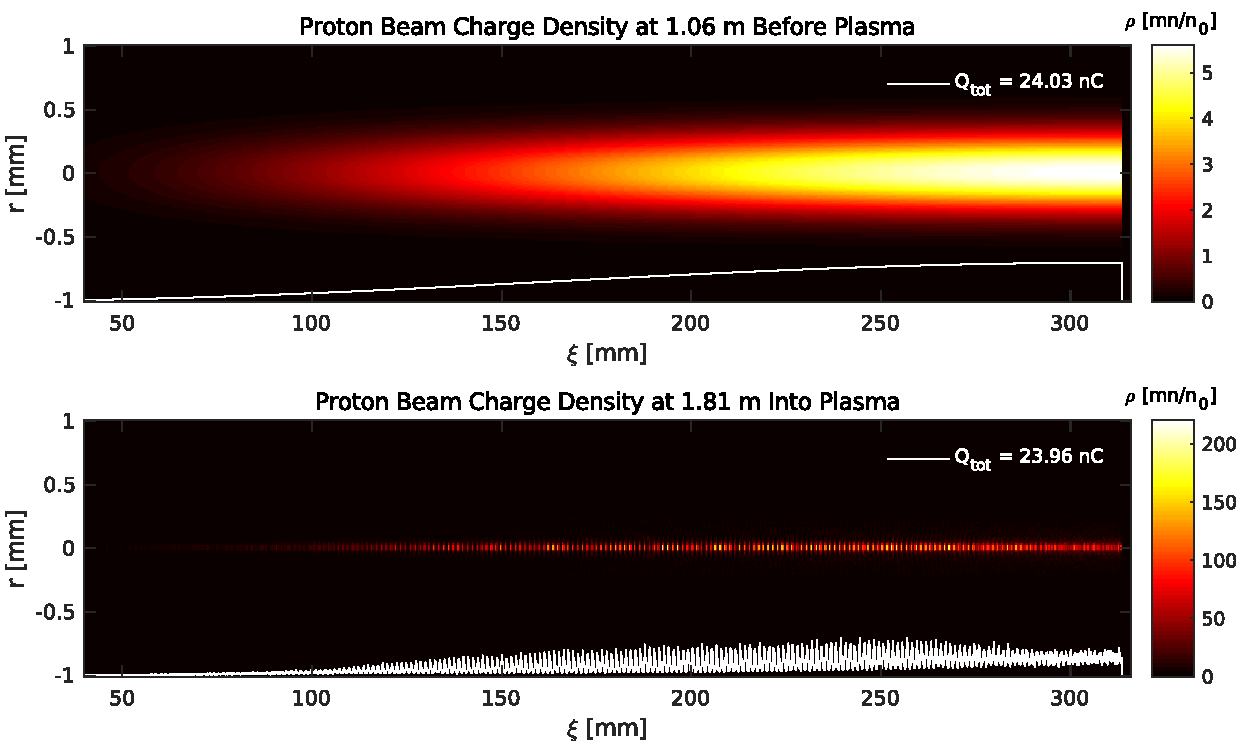
\includegraphics[width=1.0\linewidth]{figures/SelfModulationSim}
    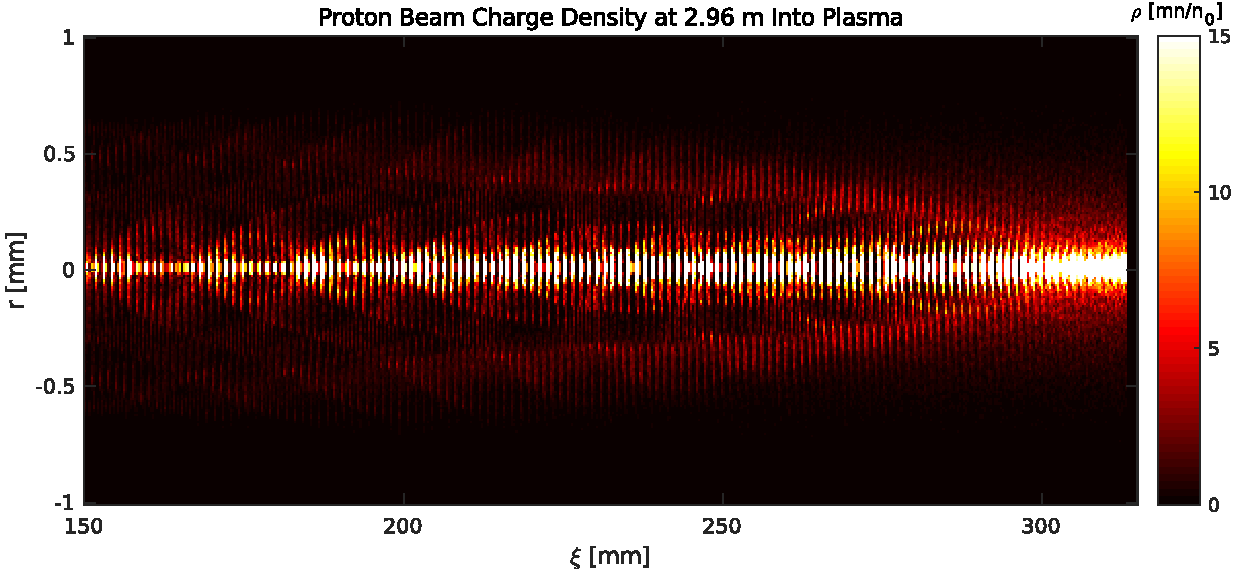
\includegraphics[width=1.0\linewidth]{figures/PBSelfModulation}
    \caption{\label{Fig:Sim:SMI} }
\end{figure}

% ================================================================================================================================ %
%  Beam Loading and Energy Spread
% ================================================================================================================================ %
\section{Beam Loading and Energy Spread}
\label{Sim:BLoad}

The transverse size of the beam was chosen to be $\sigma_{x,y}=105\unit{\mu m}$, see Table \ref{T:AWAKE-Run2}.
The longitudinal size was chosen to be $\sigma_{z}=40\unit{\mu m}$ for the studies included in Publication \ref{Pub:IPAC15}, but several lengths were tested in simulations.
$40\unit{\mu m}$ is a good compromise between having a short enough bunch to stay within the accelerating region of the accelerating wakefield, $\approx \lambda_{pe}/4$ (see Section \ref{Int:BPI:BLoad}).

% ================================================================================================================================ %
%  Emittance Evolution
% ================================================================================================================================ %
\section{Emittance Evolution}
\label{Sim:Emitt}

Emittance is preserved in the linear regime

% ================================================================================================================================ %
\subsection{The Quasi-Linear Regime}
\label{Sim:QLin}

Text

% ================================================================================================================================ %
\subsection{The Quasi-Linear + Non-Linear Case}
\label{Sim:QLinNonLin}

Quasi-linear reference \cite{rosenzweig:2010}.

An electron beam matched to the typical AWAKE plasma density will be, as discussed in \ref{Int:BPI:Match}, very narrow. At a typical normalised emittance of $2.0\unit{\mu m}$ the beam is $5.25\unit{\mu m}$. Even at low beam charge and at the upper limit in terms of beam length, the wakefields of such a beam will quickly reach the non-linear regime. In the base case used in the beam loading study included in Publication \ref{Pub:BL17} \cite{berglyd_olsen:2018} the peak density of the beam $n_b/n_0 > 35$, well beyond the saturation level of the bubble that occurs when $n_b/n_0 > 10$ \cite{lu:2005}.

The implication here is that there is an additional beneficial effect of loading the accelerating field with as much charge as it will allow without overloading it. The resulting non-linear wake driven by the head of the beam, which will see emittance growth due to the quasi-linear conditions of the proton wake, ensures that the rest of the beam sees a strong focusing force preventing further emittance growth. As the electron beam gains energy, its transverse size will decrease as its emittance is preserved as $\sigma_{r} = \sqrt{\emitN\beta}$ \cite{wille:2001}.

% ================================================================================================================================ %
\subsection{Convergence Scan}
\label{Sim:Converge}

For the large parameter scans performed for Publication~\ref{Pub:BL17}, it was necessary to verify that the results were not dependant on grid resolution.
The radial wakefields within the plasma bubble are linear, but so are the fields within one grid cell as they are interpolated on the grid.
The effect of linear focusing could thus be an artefact of resolution.
Especially in the case where the grid cells were only a factor $2.5$ smaller than the bunch $\sigma_{x,y}$, and thus the bubble radius also small.\todo{Verify and cite.}

\begin{table}[hbt]
    \centering
    \caption{Convergence results for a reference simulations for Publication~\ref{Pub:BL17}.
    The reference bunch has a charge of $250\unit{pC}$, and the emittance tolerance criterion for the $\tilde{Q}$ parameter is $5\%$ (see Section~\ref{Sim:Analysis:QTilde}).}
    \label{T:Converg}
    \begin{tabularx}{132mm}{Xl d{1}l d{1}l d{1}l}
        \rowcolor{tblhead}
        \texthh{Length} & \texthh{Param.}
            & \multicolumn{2}{c}{\texthh{1024$\times$1024}}
            & \multicolumn{2}{c}{\texthh{2048$\times$2048}}
            & \multicolumn{2}{c}{\texthh{4096$\times$4096}} \\
        \hline
                         & $\tilde{Q}$ &  213.9 & $\unit{pC}$  &  206.9 & $\unit{pC}$  &  213.1 & $\unit{pC}$  \\
        $40\unit{\mu m}$ & MEAN$(E)$   & 2263   & $\unit{MeV}$ & 2233   & $\unit{MeV}$ & 2247   & $\unit{MeV}$ \\
                         & STD$(E)$    &  267.4 & $\unit{MeV}$ &  250.4 & $\unit{MeV}$ &  261.5 & $\unit{MeV}$ \\
        \hline
                         & $\tilde{Q}$ &  221.6 & $\unit{pC}$  &  222.0 & $\unit{pC}$  &  222.1 & $\unit{pC}$  \\
        $60\unit{\mu m}$ & MEAN$(E)$   & 2346   & $\unit{MeV}$ & 2336   & $\unit{MeV}$ & 2333   & $\unit{MeV}$ \\
                         & STD$(E)$    &  166.8 & $\unit{MeV}$ &  165.0 & $\unit{MeV}$ &  165.5 & $\unit{MeV}$ \\
        \hline
                         & $\tilde{Q}$ &  229.9 & $\unit{pC}$  &  226.9 & $\unit{pC}$  &  224.8 & $\unit{pC}$  \\
        $80\unit{\mu m}$ & MEAN$(E)$   & 2378   & $\unit{MeV}$ & 2379   & $\unit{MeV}$ & 2368   & $\unit{MeV}$ \\
                         & STD$(E)$    &  120.0 & $\unit{MeV}$ &  117.6 & $\unit{MeV}$ &  119.1 & $\unit{MeV}$ \\
    \end{tabularx}
\end{table}

% ================================================================================================================================ %
\section{Optimising the Witness Beam}
\label{Sim:Opt}

Bringing it all together.

% ================================================================================================================================ %
\section{Overview of Simulation Studies}
\label{Sim:Summary}

\begin{table}[hbt]
    \centering
    \caption{Overview of total simulation cost. $97\%$ of the simulations were run on the supercomputer \textit{Abel}, on Oct Core Intel Xeon E5-2670 CPUs. The remainder were run on older nodes with Quad Core AMD Opteron 2354 CPUs.}
    \label{T:SimCost}
    \begin{tabularx}{\textwidth}{Xlrrr}
        \rowcolor{tblhead}
        \texthh{Topic of Studies}                & \texthh{Code} & \texthh{Count} &     \texthh{CPU Time} &  \texthh{Average} \\
        \hline
        Preliminary studies (mostly testing)     & OSIRIS        &           $21$ &    $266\,599\unit{h}$ & $12\,695\unit{h}$ \\
        Full length AWAKE proton bunch studies   & OSIRIS        &           $38$ &    $440\,583\unit{h}$ & $11\,594\unit{h}$ \\
        Pre-modulated beam studies$^{1}$         & OSIRIS        &          $144$ &    $319\,093\unit{h}$ &  $2\,216\unit{h}$ \\
        3D reference studies                     & OSIRIS        &           $23$ &    $245\,974\unit{h}$ & $10\,695\unit{h}$ \\
        Single drive bunch studies$^{2}$         & OSIRIS        &          $124$ &     $47\,837\unit{h}$ &     $386\unit{h}$ \\
        Beam loading and emittance studies$^{3}$ & QuickPIC      &          $293$ &    $369\,887\unit{h}$ &  $1\,262\unit{h}$ \\
        \hline
        \rowcolor{tblfoot}
        Total                                    &               &          $657$ & $1\,479\,350\unit{h}$ &  $2\,252\unit{h}$ \\
        \multicolumn{5}{p{50mm}}{\footnotesize
            $^{1}$ Main studies for Publication \ref{Pub:IPAC15} \newline
            $^{2}$ Main studies for Publication \ref{Pub:NAPAC16} \newline
            $^{3}$ Main studies for Publication \ref{Pub:BL17} \newline
        }
    \end{tabularx}
\end{table}

% ================================================================================================================================ %
